%%%%%%%%%%%%%%%%%%%%%%%%%%%%%%%%%%%%%%%%%%%%%%%%%%%%%%%%%%%%%%%%%%%%%%%
%%%%%%%%%%%%%%%%%%%%%%%%%%%%%%%%%%%%%%%%%%%%%%%%%%%%%%%%%%%%%%%%%%%%%%%
%%%%%                                                                 %
%%%%%     <file_name>.tex                                             %
%%%%%                                                                 %
%%%%% Author:      <author>                                           %
%%%%% Created:     <date>                                             %
%%%%% Description: <description>                                      %
%%%%%                                                                 %
%%%%%%%%%%%%%%%%%%%%%%%%%%%%%%%%%%%%%%%%%%%%%%%%%%%%%%%%%%%%%%%%%%%%%%%
%%%%%%%%%%%%%%%%%%%%%%%%%%%%%%%%%%%%%%%%%%%%%%%%%%%%%%%%%%%%%%%%%%%%%%%

\chapter{Background}
 %%% Give an overview of the content of the section
		Overview of the content, to be redacted
 %%%
\section{Hero}
	% Get the paragraph from the introduction
	The \gls{hero} platform is an heterogeneous system available in different configurations. 
	This platform is composed of a hard macro multicore ARM 64 Juno \gls{soc} (composed of two Cortex A57 and four Cortex A53 cores) and up to eight \gls{pulp} clusters (each of them using up to eight RI5CY cores~\cite{Art:Hero}), running on an \gls{fpga}(a Xilinx ZYNC ZC706).
	\Gls{pulp} is a \gls{cpu} based on the \gls{riscv} \gls{isa}, an open source \gls{isa} designed to support a wide range of platform from embedded systems to supercomputer.
	The modularity of the \gls{isa} makes it an interesting for \glspl{pcma} as the core are designed to support only the useful instruction for the task we want to run, which make them small and energy efficient.

	The system is also available with a Ariane \gls{riscv} 64 bits core, or just as an independant \gls{pulp} cluster for hardware simulation.


	%Sotware stack on simulation then on the fgpa platform
	Hero also has a fully functionnal software toolchain with ``support for \gls{openmp}, a linux driver and runtime librarie for both the fost and the \gls{pcma}''~\cite{Art:Hero}. The toolchain uses \texttt{clang}, a C compiler frontend of \gls{llvm}.
	The heterogeneous compiling is done by separately compiling the part of the code and then bundling together inside a single binary the two compiled file during the linking phase of the host~\cite{Report:SoftwareStack}. The final binary uses the host \gls{isa}, and embed the \gls{pcma} code in dedicated sections of the binary.





\section{Halide Language}
	\subsection { Programing model}
		Halide is a functional programming language embedded into C++, designed to write high performance image and array-processing code~\cite{Web:Halide}. This language uses a functional paradigm to describe the processing pipeline, and dissociate the array-processing code from its schedule (how the code will be compiled and run on the system). 


		Every pipeline is a function (\texttt{Halide::Func}) built using other functions and expressions (\verb|Halide:expr|) or variables (\texttt{Halide::Vars}).
		The code listing~\ref{code:simple_pipeline} describe a basic pipeline which computes the distance of each coordinate of a two-dimensional array from a given position\texttt{(center\_x, center\_y)}. 
		The creation of the pipeline is straightforward, we only need to write the desired operation using the variable \verb|x| and \verb|y|. During the execution of the pipeline or it's compilation, Halide will bound \verb|x| and \verb|y| according to the size of the output.
\lstset{basicstyle=\ttfamily\footnotesize,breaklines=true,tabsize=2}
\begin{lstlisting}[caption={Simple Pipeline Example}, captionpos=b, label={code:simple_pipeline}]
	Halide::Var x, y;
	Halide::Param center_x, center_y;
	Halide::Expr offset = Halide::pow(x - center_x, 2) 
                      + Halide::pow(y - center_y, 2);

	gradient(x, y) = offset;
\end{lstlisting}

	This simple pipeline only has one stage, but it is possible to create multi-stage pipelines and schedule them as desired. They can be transformed into a single-stage inlined pipeline or kept as is.
	The different stages can be scheduled to start as soon as they have enough data, or wait for the previous one to finish before starting to compute.

	Scheduling is done via basic scheduling primitives implemented by Halide.
The primitives consist of basic code transformations such as loop unrolling or reordering, loop splitting or merging variable together into a single one. More advanced instructions like parallelization or vectorization are also available. These instructions can be combined as needed to create complex schedules.
Section ~\nameref{section:scheduling} explain the most important scheduling instructions in greater details. 


	The listing~\ref{code:simple_pipeline_schedule} shows how schedule are designed.

	All instructions are a function of the pipeline object, they can be executed on any variable of the  pipeline. Some instructions need the variables to be bounded (e.g. the vectorize instruction) before using them.
	The scheduling primitives can be combined as needed, and the programmer can also create intermediate variables via those primitives to control precisely the execution of the code.


	\begin{lstlisting}[caption={Simple Pipeline Example}, captionpos=b,label={code:simple_pipeline_schedule}];
	gradient.parallel(x);
	gradient.unroll(y, 10);
	\end{lstlisting}

	In the listing~\ref{code:simple_pipeline_schedule},
 	Halide creates one task per value of \verb|x|. These tasks will be executed in parallel on all the cores of the system. Every task will execute a single loop over the \verb|y| axis, but instead of computing only one value of the output of the pipeline per iteration, the task will compute ten values per iteration.


	The pipeline can be translated or compiled by Halide to be executed directly on the compilation computer or in another application.
	The pipeline can be immediatly executed using the function \texttt{.realize(x\_max, y\_max)}. If an output buffer of the correct size is provided, Halide will execute the pipeline over the rectangular domain \texttt{(0,0),(x\_max,y\_max)}.
	 As halide was designed primarly to work with different hardware platform, the  cross-compilation process  has been simplified, and the pipeline can be translated to other languages.
	 Halide support translation to C code, \gls{llvm} assembly file, or already compiled object file specific to a given target(\gls{cuda}, ARM, \gls{riscv}, \gls{mips}, PowerPc...), and a given Operating Systems( Linux, Mac, Windows, Android). The pipeline can also be exported as a static library to use in another application.

\subsection{Debugging Options}

	Halide provides tools to debug the pipelines, and debugging tips to help the developers \cite{Web:HalideDebug}.

	The \texttt{print} instructions prints the value of a variable at any point of the pipeline, \texttt{print\_when()} only print when a boolean condition is True.

	The  \verb|.trace_store()| function keeps a trace of every function evaluation during execution, as long as the function hasn't been inlined, the parameters and the result of the function call will be stored in the trace and printed after the exeuction.

	Halide can print more information on the screen during the compilation of the source code by setting the environemental variable \verb|HL_DEBUG_CODEGEN| to 1. Halide will output information about every stages of the compilation and a pseudo code representation of the pipeline loops. 
	Finally, variables and functions can be labeled. Halide will replace the generic name of the variable with the label when printing the pseudo code or when using gdb.

\subsection {Basic Scheduling Options}
	\label{section:scheduling}
	Every Halide schedule applies a simple modification to the source code. Every instruction affects one or multiple variables. There are no limitation to the complexity of the schedule or the number of variable inside a pipeline.

\newcommand\EIW{.4\textwidth}
\newcommand\ECW{\textwidth - \EIW}

	\subsubsection{Default Schedule}


\begin{figure}[h]
		\begin{minipage}[c]{\EIW}
			\centering
		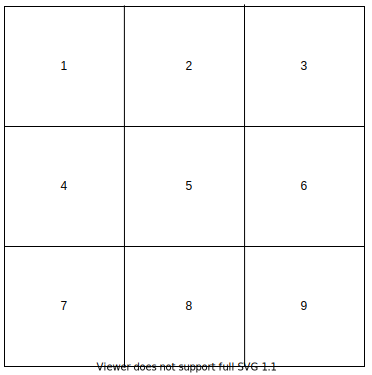
\includegraphics[width=\textwidth]{Images/BaseOrder.png}
		\end{minipage}
		\begin{minipage}[c]{\ECW}
			\centering
\begin{lstlisting}[label={code:reorder}];
			
	# Generated loops
	for(int y = 0; y < 3; y++){
		for(int x = 0; x < 3; x++){
			do something on (x,y)
		}
	}
	
\end{lstlisting}
		\end{minipage}
	\caption{Base Schedule}
	\label{schedule:default}
\end{figure}



	If no schedule is specified, Halide will evaluate the pipeline in the same order as it's arguments. The first variable being the inner most loop, and the last one the outer most loop. In figure~\ref{schedule:default}, Halide will compute the output of the pipeline in a row major fashion.

	\subsubsection{Reorder}

\begin{figure}[H]

		\begin{minipage}[c]{\EIW}
			\centering
		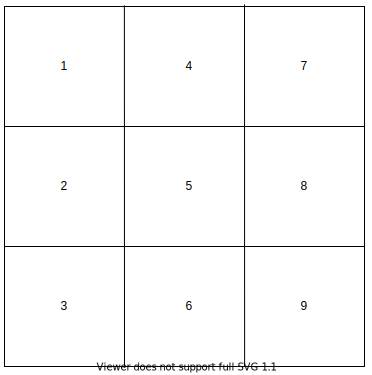
\includegraphics[width=\textwidth]{Images/Reorder.png}
		\end{minipage}
		\begin{minipage}[c]{\ECW}
			\centering
\begin{lstlisting}[label={code:reorder}];
    pipeline.reorder(y,x);


	# Generated loops
	for(int x = 0; x < 3; x++){
		for(int y = 0; y < 3; y++){
			do something on
			(x,y)
		}
	}
\end{lstlisting}
		\end{minipage}
		\caption{Schedule: Reorder}
		\label{schedule:reorder}
\end{figure}
	
	The \texttt{.reorder} instruction reorders the variable to have the given nesting order, starting from the innermost. In the figure~\ref{schedule:reorder}, the  array is now processed in a column major fashion.

	\subsubsection{Fuse}


\begin{figure}[H]

		\begin{minipage}[c]{\EIW}
			\centering
		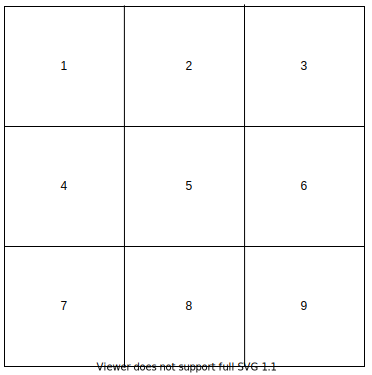
\includegraphics[width=\textwidth]{Images/BaseOrder.png}
		\end{minipage}
		\begin{minipage}[c]{\ECW}
			\centering
\begin{lstlisting}[label={code:reorder}];
    pipeline.fuse(x,y,xy);


	# Generated loops
	for(int xy = 0; xy < 9; xy++){
		do something on
		(xy)
	}
\end{lstlisting}
		\end{minipage}
		\caption{Schedule: Fused}
		\label{schedule:fuse}
\end{figure}

	The \verb|.fused| instruction fuses two dimensions together, transforming a two-dimensionnal array into a one-dimensionnal array. 


\subsubsection{Split}

\begin{figure}[H]

		\begin{minipage}[c]{\EIW}
			\centering
		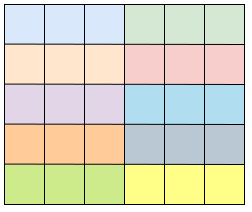
\includegraphics[width=\textwidth]{Images/Split.png}
		\end{minipage}
		\begin{minipage}[c]{\ECW}
			\centering
			\begin{lstlisting}[label={code:reorder}];
	pipeline.split(x,x_o,x_i, 3);


	# Generated loops
	for(int y = 0; y < 6; y++){
		for(int x_o = 0; x_o < 2; x_o++){
			for(int x_i = 0; x_i < 3; x_i++){
				do something on
				(x_o * 3 + x_i, y)
			}
		}
	}
\end{lstlisting}
		\end{minipage}
		\caption{Schedule Split}
		\label{schedule:split}
\end{figure}

	This schedule split a loop in an inner and an outer subdimensions, where the size of the inner dimension is specified by the last argument. This shedule is useful to cut the array in smaller pieces that will be computed in parallel or using \gls{simd} instructions.

\subsubsection{Tile}


\begin{figure}[H]

		\begin{minipage}[c]{\EIW}
			\centering
		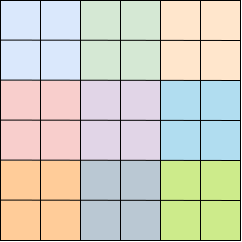
\includegraphics[width=\textwidth]{Images/Tile.png}
		\end{minipage}
		\begin{minipage}[c]{\ECW}
			\centering
			\begin{lstlisting}[label={code:reorder}];

	pipeline.split(x,y,x_o,y_o,x_i,y_i,2,2);



	# Generated loops
	for(int y_o = 0; y_o < 6; y_o++){
		for(int x_o = 0; x_o < 3; x_o++){
			for(int y_i = 0; y_i < 2; y_i++){
				for(int x_i = 0; x_i < 2; x_i++){
					do something on
					(x_o * 2 + x_i, y_o * 2 + y_i)
				}
			}
		}
	}
\end{lstlisting}
		\end{minipage}
		\caption{Schedule Tile}
		\label{schedule:tile}
\end{figure}
	The Tile schedule is similar to the Split schedule, but along two dimensions. It creates multiples smaller rectangular tiles which can be processed independently.

	\subsubsection{Unroll}


\begin{figure}[H]
		\begin{minipage}[c]{\EIW}
			\centering
		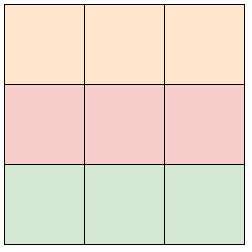
\includegraphics[width=\textwidth]{Images/Unroll.png}
		\end{minipage}
		\begin{minipage}[c]{\ECW}
			\centering
			\begin{lstlisting}[label={code:reorder}];



	# Generated loops
	pipeline.unroll(x,3);
	for(int y = 0; y < 4; y++){
		do something on (0,y)
		do something on (1,y)
		do something on (2,y)
	}

\end{lstlisting}
		\end{minipage}
	\caption{Unroll Schedule}
	\label{schedule:unroll}
\end{figure}
	The Unroll schedule unrolls the code along one dimension. This technique is often used when multiple computations share the same data, to prevent multiple memory access. In the figure~\ref{schedule:unroll}, we first  split the x dimension before unrolling as Halide can't unroll a variable if it isn't bounded.

\subsubsection{Parallel}
\begin{figure}[H]

		\begin{minipage}[c]{\EIW}
			\centering
		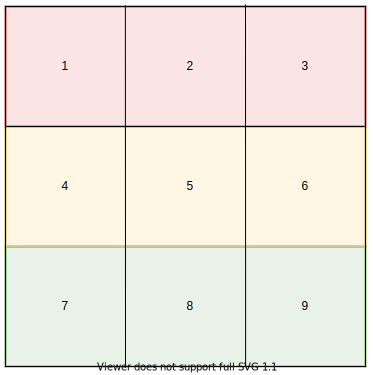
\includegraphics[width=\textwidth]{Images/Parallel.png}
		\end{minipage}
		\begin{minipage}[c]{\ECW}
			\centering
			\begin{lstlisting}[label={code:reorder}];
	pipeline.parallel(y);
	# Core 0: y = 0 for(int x = 0; x < 4; x++){
		do something on (x,0)
	}

	# Core 1: y = 1
	for(int x = 0; x < 4; x++){
		do something on (x,1)
	}

	# Core 2: y = 2
	for(int x = 0; x < 4; x++){
		do something on (x,2)
	}
	}
\end{lstlisting}
		\end{minipage}
		\caption{Schedule Parallel}
		\label{schedule:parallel}
\end{figure}


The parallel schedule distributes the pipeline to all the available cores.

In the example~\ref{schedule:parallel}, the code is distributed on three cores, each of them execute a single loop along the y axis.

Halide will create a task for each value the variable can take, and these tasks will be executed with the \texttt{halide\_do\_par\_for} function. This function needs to be overwritten on \gls{hero} to distribute the tasks on the \gls{pulp} cluster. 


	\subsubsection{Vectorize}
	The goal of this schedule is to setup the code so to make use of the \gls{simd} instructions of the \gls{cpu}. Currently, \gls{llvm} doesn't support the vector extension  implemented in the \gls{pulp} cluster, but the generated code will take advantages of all the registers available to compute the output values, and try to compute multiple values at the same time.


	\subsection { Porting Halide to new Platforms}

	In order to compile Halide, we need to compile \gls{llvm} with the flag without shared libraries otherwise, Halide won't compile, and  with support for the desired targets (x86, \gls{riscv} and \gls{aarch64}).

	The library header file generated by Halide explains which functions needs to be implemented to make Halide work on our target platform.
	The error messages during the linking phase are also a good source of information to find which function are needed to compile the code. 

	To make Halide work on \gls{hero}, we only need to port a few subset of functions. As most of the schedule are only reformatting the code, only the parallel schedule has platform specific code. So we can make Halide work with this specific code, the memory allocation primitives and the debugging functions (\texttt{halide\_printf}).



		

%%% Local Variables: 
%%% mode: latex
%%% TeX-master: "../report_template"
%%% End: 
